% LaTeX source for ``การเรียนรู้ของเครื่องสำหรับเคมีควอนตัม (Machine Learning for Quantum Chemistry)''
% Copyright (c) 2022 รังสิมันต์ เกษแก้ว (Rangsiman Ketkaew).

% License: Creative Commons Attribution-NonCommercial-NoDerivatives 4.0 International (CC BY-NC-ND 4.0)
% https://creativecommons.org/licenses/by-nc-nd/4.0/

\chapter{ลักษณะเฉพาะของอะตอมและโมเลกุล}
\label{ch:feature}

\begin{figure}[htbp]
    \centering
    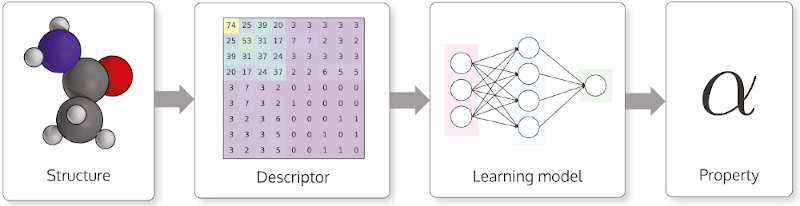
\includegraphics[width=\linewidth]{fig/workflow_chem_ml.png}
    \caption{ขั้นตอนแสดงการสร้างโมเดลการเรียนรู้ของเครื่องเพื่อใช้ในการทำนายคุณสมบัติของโมเลกุล เริ่มจากการเปลี่ยนข้อมูลทางเคมีจาก%
    จากโครงสร้างของโมเลกุลไปเป็นข้อมูลแบบดิจิทัลที่คอมพิวเตอร์สามารถเข้าใจและประมวลผลต่อได้ ตามด้วยขั้นตอนการสร้างโมเดลสำหรับ%
    การเรียนรู้ และขั้นตอนสุดท้ายคือการทำนายคุณสมบัติของโมเลกุล (เครดิตภาพ: https://chemintelligence.com)}
    \label{fig:workflow_chem_ml}
\end{figure}

ในบทนี้เราจะมาดูความสำคัญของลักษณะเฉพาะ (Feature) ของโมเลกุลต่อประสิทธิภาพของโมเดล ML ในการทำนายคุณสมบัติของโมเลกุล ซึ่งการ%
คำนวณ Feature เป็นหนึ่งในขั้นตอนที่สำคัญมากของ ML ดังแสดงในภาพที่ \ref{fig:workflow_chem_ml} ซึ่งแสดงขั้นตอน (Workflow) 
ในการสร้างโมเดลเพื่อเชื่อมโยงความสัมพันธ์ระหว่างโครงสร้างของโมเลกุลกับคุณสมบัติทางเคมีของโมเลกุลนั้น ๆ จะเห็นได้ว่าทั้งสองอย่างนี้จริง ๆ 
แล้วมีความเชื่อมโยงกันผ่านโครงสร้างเชิงอิเล็กทรอนิกส์ (Electronic Structure) แต่ว่าความสัมพันธ์นั้นมีความซับซ้อนและการที่จะหาสมการทาง%
คณิตศาสตร์ที่อธิบายความเชื่อมโยงนี้ได้นั้นเป็นเรื่องอาจจะทำได้ไม่ง่ายนัก ซึ่งปัญหาตรงนี้ ML ก็ได้เข้ามาช่วยในฐานะที่เป็นเครื่องมือหนึ่งที่พยายามสร้าง%
สมการทางคณิตศาสตร์ในรูปแบบของฟังก์ชันที่ขึ้นอยู่กับตัวแปรที่อ้างอิงกับรูปแบบที่เกิดจากข้อมูลภายในชุดข้อมูลขนาดใหญ่โดยเชื่อมโยงผ่าน Feature 
นั่นเอง
\idxboth{โครงสร้างเชิงอิเล็กทรอนิกส์}{Electronic Structure}

Feature หรือ Representation คือคุณลักษณะที่บ่งบอกความเฉพาะตัวของอะตอมหรือโมเลกุลนั้น ๆ ซึ่งอาจจะเรียกว่าเป็นคุณลักษณะแบบพิเศษ 
(Special Attributes) ก็ได้ นอกจากนี้เราสามารถตีความได้ว่า Feature นั้นจริง ๆ แล้วก็เปรียบเสมือนเป็นตัวแทนของสิ่งที่เราสนใจอีกด้วย 
ซึ่งในบริบททางเคมีนั้นเราจะเรียกสิ่งที่เป็นตัวแทนของโมเลกุลว่า Molecular Representation อย่างไรก็ตามผู้เขียนมีความเห็นว่าจริง ๆ แล้ว 
Feature กับ Representation ก็ไม่ได้มีความหมายเหมือนกันเสียทีเดียว ขึ้นอยู่กับประเภทของข้อมูลที่ใช้เป็น Feature แต่ผู้เขียนจะใช้คำว่า 
Representation ในการอ้างถึงลักษณะเฉพาะของระบบที่เรากำลังศึกษา (อะตอม, โมเลกุล, และสารประกอบ) เพราะว่าให้ความหมายที่สื่อ%
การเป็นตัวแทนของระบบที่เราสนใจได้ดีกว่า\autocite{stepisnik2021}
\idxboth{ลักษณะเฉพาะ}{Feature}
\idxboth{ตัวแทนของโมเลกุล}{Molecular Representation}
\idxboth{ตัวแทน}{Representation}

การแบ่งประเภทของ Feature หรือ Representation ในทางเคมีนั้นสามารถแบ่งได้หลายประเภท ขึ้นอยู่กับเกณฑ์ที่จะใช้ในการแบ่ง ความคิดเห็น%
ส่วนตัวของผู้เขียนก็คือเราสามารถแบ่ง Feature ได้อย่างง่ายที่สุดเลยก็คือแบ่งตามสเกลของความจำเพาะเจาะจงของ Feature ที่คำนวณมาจาก%
โมเลกุล กล่าวคือการที่เราต้องการที่จะทำนายคุณสมบัติของโมเลกุลนั้น เราควรจะต้องทราบก่อนว่าคุณสมบัติของโมเลกุลชนิดนั้นอยู่ในสเกลไหน 
โดยสเกลในที่นี้แบ่งง่าย ๆ เป็นระดับเฉพาะที่ (Local) หรือแบบทั่วทั้งพื้นที่ (Global) ตัวอย่างเช่น พลังงานรวมของโมเลกุลกับความสามารถใน%
การละลายในน้ำเป็นคุณสมบัติในระดับ Global เพราะว่าแต่ละโมเลกุลมีค่าเหล่านี้ได้เพียงแค่หนึ่งค่าเท่านั้น แต่ถ้าหากเป็นคุณสมบัติอย่างเช่นแรงเชิง%
อะตอมหรือประจุย่อย คุณสมบัติเหล่านี้จะถูกจัดให้เป็นคุณสมบัติระดับ Local เพราะว่าอยู่ในสเกลระดับอะตอม เมื่อเราทราบแล้วว่าคุณสมบัติของเรา%
เป็นแบบ Local หรือ Global เราก็สามารถที่จะพิจารณาเลือก Feature ที่อยู่ในระดับเดียวกันเพื่อมาใช้ในการฝึกสอนโมเดลได้ เพราะการที่เรา%
ใช้ Feature ที่อยู่ในระดับเดียวกับเอาต์พุตที่ต้องการทำนายนั้นจะทำให้การหาความสัมพันธ์ระหว่างสองสิ่งนี้ทำได้ง่ายและสมเหตุสมผล
\idxboth{ลักษณะเฉพาะ!แบบเฉพาะที่}{Feature!Local}
\idxboth{ลักษณะเฉพาะ!แบบทั่วทั้งพื้นที่}{Feature!Global}

%--------------------------
\section{ความสำคัญของลักษณะเฉพาะ}
\label{sec:why_feature}
%--------------------------

คำถามที่ตามมาก็คือ \enquote{\textit{Molecular Representation มีความสำคัญมากไหม และมีความสำคัญอย่างไร}} แน่นอนว่าคำตอบ%
คือต้องมีความสำคัญอยู่แล้ว (เพราะถ้าหากไม่สำคัญผู้เขียนก็คงไม่เขียนหัวข้อนี้ใช่ไหมครับ) และมีความสำคัญมากด้วย โดยส่วนตัวของผู้เขียนนั้นคิดว่า
Molecular Representation มีความสำคัญมากที่สุดเลยก็ว่าได้ เพราะ Representation ก็คืออินพุตที่เรานำมาใช้ฝึกสอนโมเดล ML นั่นเอง 
ดังนั้น Molecular Representation จึงเป็นปัจจัยหลักที่กำหนดประสิทธิภาพในการทำนายของโมเดลด้วย 

เนื่องจากว่ามนุษย์สามารถแยกแยะโมเลกุลแต่ละตัวออกจากกันได้ แต่ว่าคอมพิวเตอร์ไม่สามารถทำได้เพราะว่าคอมพิวเตอร์เข้าใจข้อมูลที่เป็นแบบดิจิทัล%
ในภาษาเครื่องจักรเท่านั้น (Machine Language) ดังนั้นเราจึงต้องมีการใช้ Representation เพื่ออธิบายโมเลกุลในรูปแบบของค่าพารามิเตอร์%
ที่คอมพิวเตอร์สามารถเข้าใจได้ เช่น แปลงโมเลกุลเป็นข้อมูลเชิงตัวเลข (Numeric) ให้อยู่ในรูปของเวกเตอร์หรือเมทริกซ์ สำหรับการอธิบายโมเลกุล%
แบบง่าย ๆ นั้นสามารถทำได้โดยใช้ Representation เพื่อมาอธิบายข้อมูลเชิงโครงสร้าง (Structural Properties) ซึ่งสามารถใช้ข้อมูลทาง%
เคมีทั่วไปได้ ยกตัวอย่างเช่น รูปร่างของโมเลกุล, จำนวนหมู่ฟังก์ชัน, ชนิดของพันธะระหว่างอะตอมคาร์บอน, และจำนวนวงเบนซีน ฯลฯ ซึ่งข้อมูล%
เหล่านี้เราสามารถคำนวณออกมาได้ง่าย ๆ ไม่มีความซับซ้อนอะไร แต่ปัญหาคือ Representation ที่เป็น Structure-based นั้นมีข้อมูลที่น้อยเกินไป 
จึงทำให้ไม่สามารถถูกนำมาใช้เป็นอินพุตสำหรับการสร้างโมเดลเพื่อทำนายคุณสมบัติหรือพารามิเตอร์ทางเคมีที่ซับซ้อนหรือละเอียดกว่าได้ เช่น 
พลังงานพันธะ (Bond Energy), พลังงานของออร์บิทัล (Orbital Energy), ความถี่เชิงการสั่น (Vibrational Frequency), ไดโพลโมเมนต์ 
(Dipole Moment), ฯลฯ นั่นก็เพราะว่าอินพุตของเราเป็น Representation ที่ไม่มีความสัมพันธ์กับเอาต์พุตที่เราต้องการทำนาย (จริง ๆ ก็อาจจะ%
สอดคล้องแต่ว่าไม่ได้สอดคล้องกันแบบโดยตรง)

\begin{figure}[htbp]
    \centering
    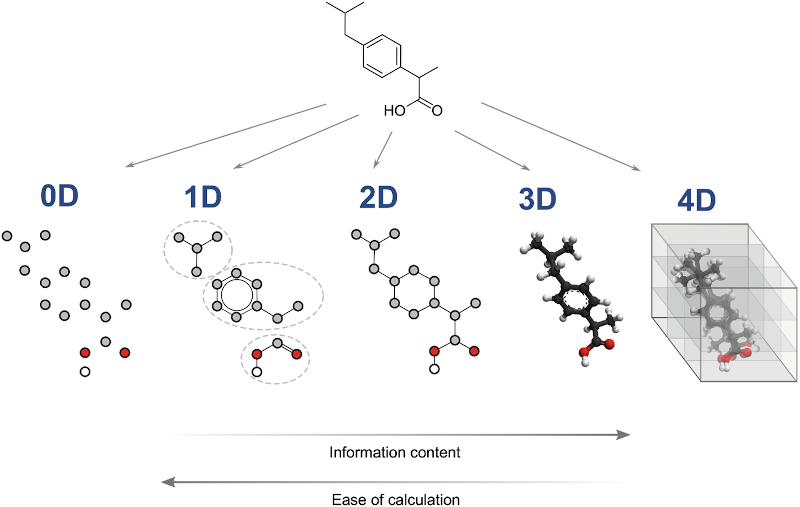
\includegraphics[width=\linewidth]{fig/descriptor_classes.png}
    \caption{แผนภาพแสดงการแบ่งประเภทของ Descriptor หรือตัวคำนวณคุณลักษณะเฉพาะของโมเลกุลโดยแบ่งตามจำนวนมิติของโมเลกุล 
    (เครดิตภาพ: https://chemintelligence.com)}
    \label{fig:descriptor_classes}
\end{figure}

ดังนั้นถ้าหากเราต้องการที่จะทำนายเอาต์พุตที่เป็นปริมาณที่มีความละเอียดอยู่ในระดับอะตอม (ปริมาณเชิงอิเล็กทรอนิกส์) เราควรจะใช้ Representation 
ที่อยู่ในระดับเดียวกันและ Representation ควรจะต้องให้ Feature Vectors ที่เก็บข้อมูลทางเคมีควอนตัมและฟิสิกส์ไว้ด้วย โดยการพัฒนา 
Representation โดยใช้องค์ความรู้ทางฟิสิกส์ (Physics-inspired Representation) ก็เป็นหนึ่งในหัวข้องานวิจัยที่กำลังมาแรงในขณะนี้ 
ข้อมูลทางฟิสิกส์ที่เราเพิ่มเข้าไปก็เปรียบเสมือนเป็นส่วนเติมเต็มที่เพิ่มความถูกต้อง (เรียกอีกอย่างว่าการทำ Correction) ให้กับ Representation 
มากขึ้น โดยเราสามารถใส่ความเป็นสมมาตร (Symmetricity) หรือคุณสมบัติจากปรากฎการณ์ทางฟิสิกส์เชิงควอนตัมของโมเลกุลเข้าไปได้ เป็นต้น 
\idxboth{ความเป็นสมมาตร}{Symmetricity}

%--------------------------
\section{การแปลงข้อมูลเชิงโมเลกุล}
\label{sec:mol_transform}
\idxth{การแปลงข้อมูลเชิงโมเลกุล}
%--------------------------

\begin{figure}[htbp]
    \centering
    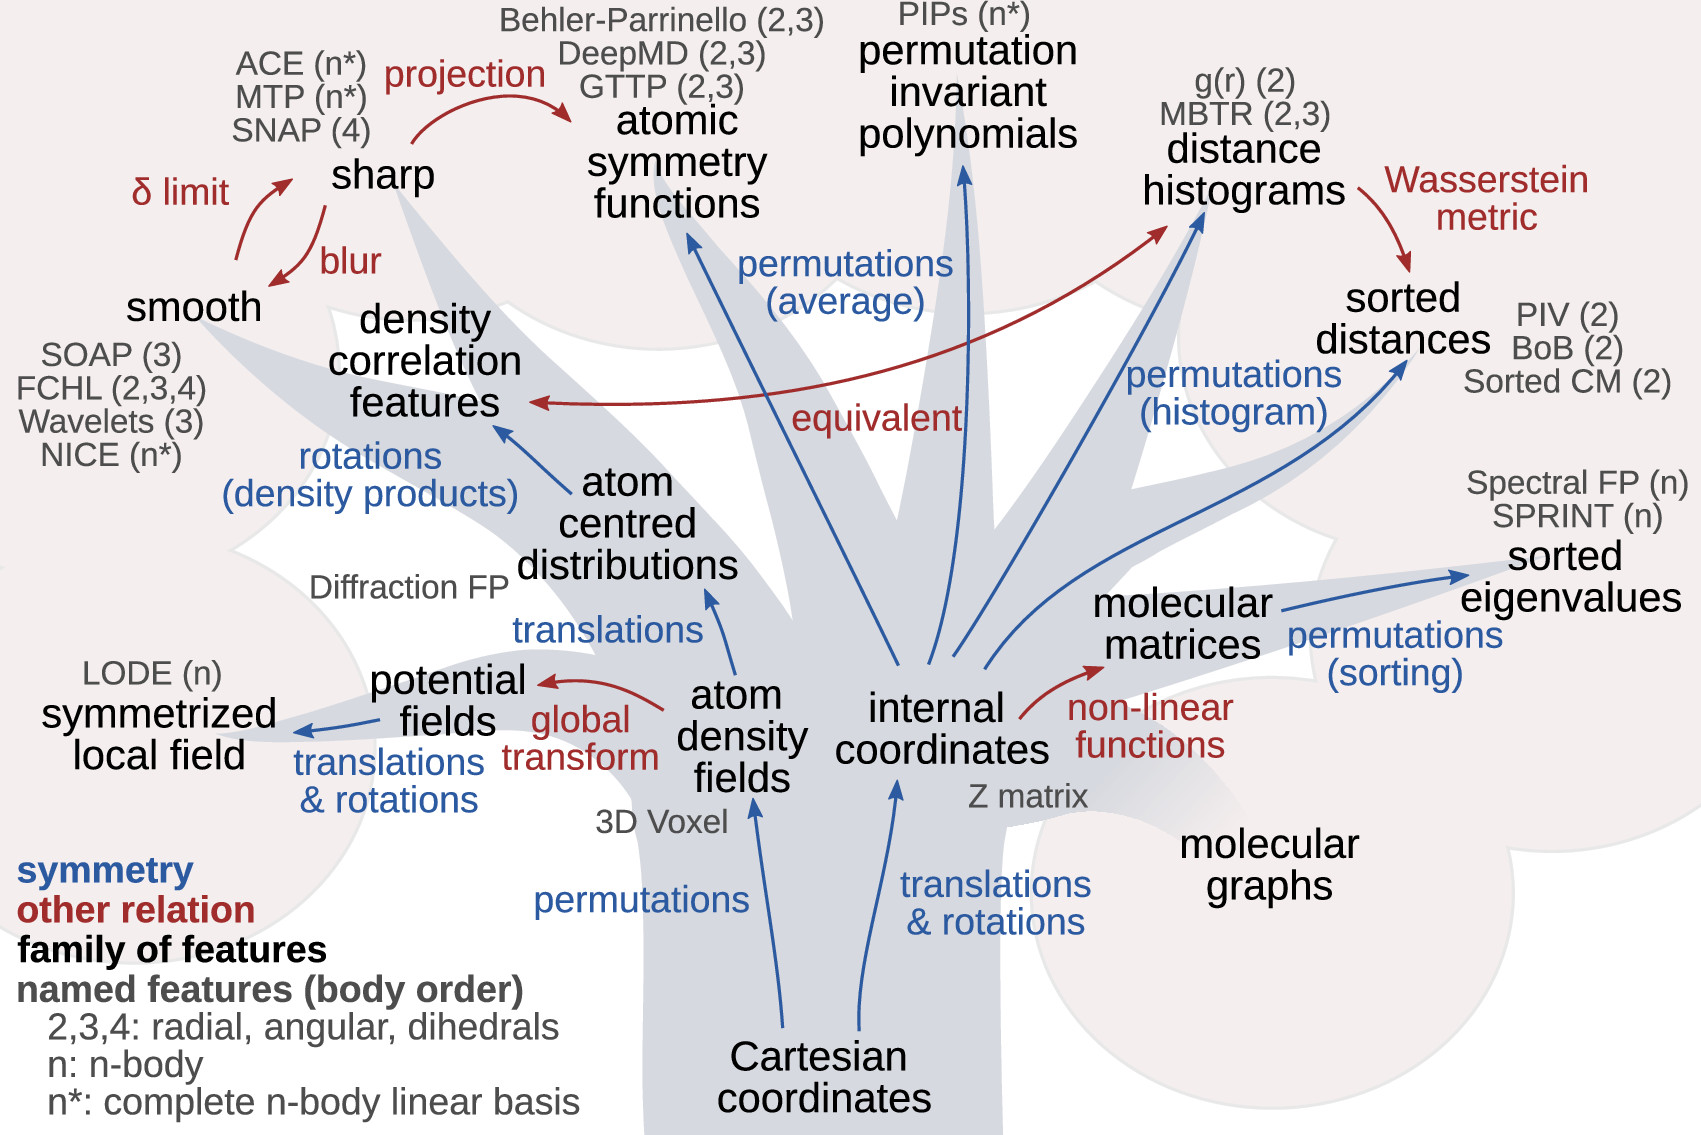
\includegraphics[width=\linewidth]{fig/qm_descriptors_map.jpeg}
    \caption{แผนผังแสดงความเชื่อมโยงของ Descriptor ทั้งเชิงโครงสร้างและอิเล็กทรอนิกส์โดยเริ่มจาก Cartesian Coordinates ของ%
    โมเลกุลแล้วพัฒนาต่อเป็น Descriptor แบบต่าง ๆ
    (เครดิตภาพ: \textit{Chem. Rev.} \textbf{2021}, 121, 16, 9759-9815\autocite{musil2021})}
    \label{fig:qm_descriptor_map}
\end{figure}

โมเลกุลประกอบไปด้วยอะตอมหลายอะตอมมารวมกัน เราจึงเปรียบเทียบโมเลกุลเป็นประโยคหรือข้อความและเปนียบเทียบอะตอมเป็นคำแต่ละคำได้
ดังที่บอกไปในข้างต้นว่าการทำให้คอมพิวเตอร์เข้าใจความเชื่อมโยงระหว่างอะตอมในโมเลกุลนั้นต้องมีการเลือกใช้ Representation ที่เหมาะสม
โดยคุณสมบัติของ Representation ที่ดีนั้นไม่เพียงแต่จะต้องไม่ขึ้นกับการเคลื่อนที่เชิงการหมุน (Rotational Motion) และการเคลื่อนที่เชิงเส้น 
(Translational Motion) เท่านั้น แต่ควรจะต้องมีความเรียบง่ายและไม่ซับซ้อนหรือยุ่งยากเกินไปในการคำนวณเพื่อสร้าง Machine Code 
จากพิกัดตำแหน่งคาร์ทีเซียน (Cartesian Coordinates) ด้วย

\begin{figure}[htbp]
    \centering
    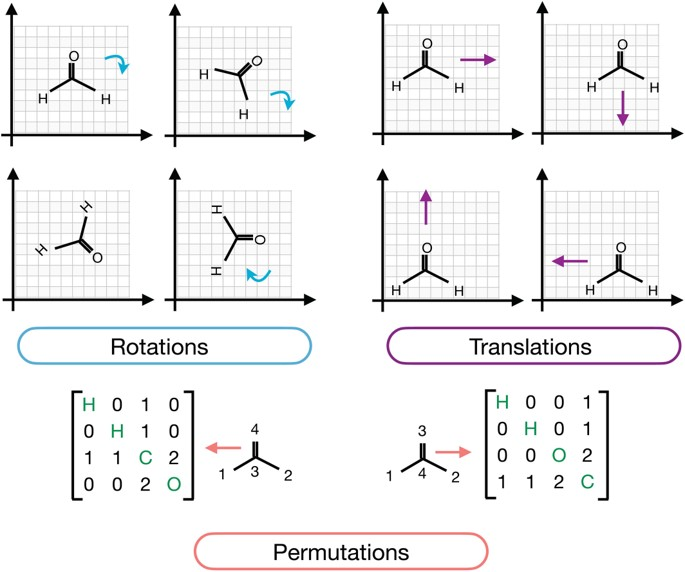
\includegraphics[width=\linewidth]{fig/mol_rep_invar.jpg}
    \caption{Invariance ของการเคลื่อนที่เชิงเส้น (Translation), การเคลื่อนที่เชิงการหมุน (Rotation) และการเปลี่ยนลำดับ
    (Permutation) ของโมเลกุล Formaldehyde}
    \label{fig:mol_rep_invariance}
\end{figure}

ภาพที่ \ref{fig:mol_rep_invariance} แสดงตัวอย่างของการเคลื่อนที่แบบต่าง ๆ รวมถึงการเปลี่ยนลำดับซึ่งคุณสมบัติเหล่านี้จะสอดคล้องกับ%
สมมาตรของโมเลกุลด้วย โดยเงื่อนไขในการพิจารณาว่า Molecular Representation ไหนมีความเหมาะสมในการนำมาคำนวณ Feature Vectors 
มีดังต่อไปนี้

\begin{enumerate}[topsep=0pt]
    \item การไม่ขึ้นกับการหมุน (Rotational Invariance): Representation จะต้องไม่ขึ้นกับโอเปอเรเตอร์ของการหมุน
    
    \item การไม่ขึ้นกับการเลื่อนตำแหน่ง (Translational Invariance): Representation จะต้องไม่เปลี่ยนไปเมื่อมีการเลื่อนตำแหน่ง%
    แบบเชิงเส้นภายในปริภูมิ
    
    \item การไม่ขึ้นกับการเปลี่ยนลำดับ (Permutation Invariance): Representation จะต้องไม่เปลี่ยนไปเมื่อมีการเปลี่ยนลำดับหรือสลับ%
    อะตอม
\end{enumerate}

%--------------------------
\section{ลักษณะเฉพาะเชิงโครงสร้างแบบทั่วไป}
\label{sec:struc_feat}
\idxth{ลักษณะเฉพาะ!เชิงโครงสร้างแบบทั่วไป}
\idxen{Representation!Structural Representation}
%--------------------------

%--------------------------
\subsection{Internal Coordinates}
\label{ssec:internal_coord}
\idxen{Representation!Internal Coordinates}
%--------------------------

พิกัดภายในของโมเลกุล (Internal Coordinates) หรือเรียกอย่างว่า $Z$ Matrix เป็น Representation พื้นฐานที่สุดในการอธิบายโครงสร้าง%
ของโมเลกุล (ไม่นับการใช้พิกัดของอะตอมแต่ละอะตอมโดยตรง) อาจจะเรียกได้ว่าเป็น Representation ที่เรียบง่ายที่สุดเลยก็ว่าได้ โดยถูกใช้อย่าง%
แพร่หลายในยุคแรก ๆ ที่มีการนำ ML มาใช้สำหรับเคมีและยังถูกใช้มาอย่างยาวนานจึงถึงปัจจุบัน ข้อดีอย่างหนึ่งของ Internal Coordinates คือ%
สามารถอธิบายได้ทั้งโมเลกุล โดยองค์ประกอบของ Representation อันนี้มีความยาวพันธะระหว่างอะตอม (Bond Distance, $d$) มุมพันธะ 
(Bond Angle, $\alpha$) และมุมบิดเบี้ยว (Dihedral Angle หรือ Torsion, $\theta$) ซึ่งอะตอมที่ถูกเลือกมาคำนวณ Internal 
Coordinates นั้นมักจะเป็นอะตอมที่เรียงติดกัน (มีพันธะเคมีระหว่างกัน) หรืออยู่ใกล้กัน อย่างไรก็ตามเราสามารถคำนวณหา Internal 
Coordinates ของโมเลกุลได้โดยพิจารณาอะตอมทุก ๆ คู่หรือทุกความเป็นไปได้ทั้งหมดภายในโมเลกุล โดยเซตของ Internal Coordinates 
สามารถเขียนได้ดังนี้

\begin{equation}\label{eq:internal_coord}
    Z = \{ d, \alpha, \theta \}
\end{equation}

%--------------------------
\subsection{Geometric Descriptors}
\label{ssec:geom_descriptor}
\idxth{ลักษณะเฉพาะ!เชิงเรขาคณิต}
\idxen{Representation!Geometric Descriptors}
%--------------------------

Geometric Descriptors (ลักษณะเฉพาะเชิงเรขาคณิต) เป็น Descriptor (จะเรียกแทนด้วย Representation ก็ได้) ที่อ้างอิงกับข้อมูล%
ตำแหน่งของอะตอมในโมเลกุล โดยมักจะเชื่อมโยงกับ Representation แบบที่เป็นสัญลักษณ์ (Symbolic Representation) เช่น SMILES ซึ่ง 
Geometric Descriptors ก็สามารถแบ่งออกเป็นได้หลาย Descriptor ซึ่งก็รวมไปถึง $Z$ Matrix, Coordination Number, Adjacency 
Matrix อย่างไรก็ตาม Representation ในกลุ่มนี้มักจะให้ผลการทำนายด้วย ML ไม่ค่อยดีนัก นั่นก็เพราะว่าความสามารถในการกักเก็บข้อมูลเชิง%
อิเล็กทรอนิกส์นั้นน้อยมากเมื่อเทียบกับ Representation ประเภทที่เป็นแบบเชิงอะตอม (Atom-wise Descriptor) และยังมีโมเลกุลบางประเภทที่ 
Geometric Descriptors ไม่สามารถนำไปใช้ได้ อย่างเช่นโมเลกุลไอโซเมอร์ เช่น cis/trans สเตอริโอไอโซเมอร์ ดังนั้น Representation 
ประเภทนี้จึงไม่เป็นที่นิยมในการนำมาฝึกสอนโมเดล ML โดยเฉพาะโมเดลที่ใช้ในงานวิจัยทางด้านเคมีควอนตัม\autocite{keith2021,musil2021}

%--------------------------
\section{ลักษณะเฉพาะเชิงโครงสร้างสำหรับโมเลกุล}
\label{sec:struc_feat_mol}
\idxth{ลักษณะเฉพาะ!เชิงโครงสร้างสำหรับโมเลกุล}
\idxen{Representation!Molecular Representation}
%--------------------------

Representation ประเภทนี้จะเป็นการอธิบายสภาพแวดล้อม (Environment) ของอันตรกิริยาระหว่างอะตอมทุกอะตอมในโมเลกุล โดยมักจะอยู่ใน%
รูปของเมทริกซ์ เช่น เมทริกซ์ของส่วนกลับของระยะห่างระหว่างอะตอม (Inverse Distance Matrix) และเมทริกซ์คูลอมบ์ (Coulomb Matrix)

%--------------------------
\subsection{Inverse Distance Matrix}
\label{ssec:inv_dist_mat}
\idxth{ลักษณะเฉพาะ!เมทริกซ์ของส่วนกลับของระยะห่างระหว่างอะตอม}
\idxen{Representation!Inverse Distance Matrix}
%--------------------------

Inverse Distance Matrix (เมทริกซ์ของส่วนกลับของระยะห่างระหว่างอะตอม) เป็น Representation Matrix แบบที่ง่ายที่สุดและมีความหมาย%
ทางเคมีที่ชัดเจน นั่นก็คือการใช้ส่วนกลับของระยะห่างระหว่างนิวเคลียสของอะตอมนั้นเป็นการจำลองเทอมของอันตรกิริยาระหว่างนิวเคลียสที่อยู่ใน 
Hamiltonian ของพลังงาน นิยามทางคณิตศาสตร์ของ Inverse Distance Matrix ($D$) อธิบายได้ตามสมการต่อไปนี้

\begin{equation}
    D_{ij} = \frac{1}{||r_{i} - r_{j}||}
\end{equation}

เมื่อเราคำนวณ Inverse Distance ออกมาเป็นเมทริกซ์ขนาด $i \times j$ แล้ว เราจะพบว่าสมาชิกของเมทริกซ์ในแนวทแยง (Diagonal 
Elements) นั้นจะไม่มีความหมาย ดังนั้นเราจึงสนใจเฉพาะสมาชิกนอกแนวทแยง (Off-diagonal Elements)

%--------------------------
\subsection{Coulomb Matrix}
\label{ssec:coulomb_mat}
\idxth{ลักษณะเฉพาะ!เมทริกซ์คูลอมบ์}
\idxen{Representation!Coulomb Matrix}
%--------------------------

Coulomb Matrix (เมทริกซ์คูลอมบ์) เป็น Molecular Representation ที่ถูกเสนอครั้งแรกในปี ค.ศ. 2012 โดย Matthias Rupp 
และทีมวิจัย\autocite{rupp2012} โดยได้ถูกนำมาใช้อย่างแพร่หลายในงานวิจัยทางด้าน ML นั่นก็เพราะว่าไม่มีความสิ้นเปลืองในการคำนวณและ%
ให้ความแม่นยำในการทำนายค่าพลังงานของโมเลกุลสูง ซึ่ง Coulomb Matrix นั้นถูกพัฒนาขึ้นมาโดยมีพื้นฐานมาจาก Inverse Distance Matrix 
ซึ่งเป็นการแก้ปัญหาที่พบใน Distance Matrix สองส่วนดังนี้

\begin{enumerate}
    \item มีการกำหนดเงื่อนไขในการคำนวณสมาชิกโดยกำหนดค่าของสมาชิกในแนวทแยง
    
    \item รวมประจุของอะตอมเข้าไปด้วย ซึ่งเป็นพารามิเตอร์สำคัญในการพัฒนา Force Field สำหรับการจำลองพลวัตเชิงโมเลกุล (Molecular 
    Dynamics หรือ MD)
\end{enumerate}

สมการสำหรับการคำนวณสมาชิกของ Coulomb Matrix คือ

\begin{equation}\label{eq:cm}
    C_{ij} =
    \begin{cases}
    \frac{1}{2} Z_i^{2.4} & \text{ if } i = j \\ 
    \frac{Z_i Z_j}{R_{ij}} & \text{ if } i \neq j
    \end{cases}
\end{equation}

จากสมการที่ \ref{eq:cm} จะเห็นได้ว่าเราได้แบ่งเงื่อนไขในการคำนวณสมาชิกของ Coulomb Matrix ออกเป็นสองเงื่อนไข สำหรับกรณีคู่อะตอม%
เหมือนกันและต่างกัน โดยที่พลังงานศักย์เชิงไฟฟ้าสถิตย์ของอะตอมแต่ละคู่นั้นจะถูกเข้ามาด้วย (ผ่านเทอมของประจุ) นั่นก็คือสมาชิกนอกแนวทแยง%
จะแสดงถึงแรงผลักคูลอมบ์ระหว่างอะตอม ในขณะที่สมาชิกในแนวทแยงจะเป็นการเทียบเคียงค่าเลขอะตอมกับพลังงานของอะตอมในกรณีที่ไม่ได้มี%
อันตรกิริยากับอะตอมตัวอื่น

ถึงแม้ว่า Coulomb Matrix จะเป็น Representation ที่ไม่ขึ้นกับการเลื่อนตำแหน่งและการหมุนของโมเลกุล แต่ว่าก็ยังขึ้นอยู่กับการเปลี่ยนตำแหน่ง%
หรือการสลับที่กันของอะตอม เพื่อแก้ปัญหาดังกล่าว ได้มีนักวิจัยได้นำเสนอ Representation ตัวใหม่อีกหลายตัวที่เปรียบเสมือนเป็น Coulomb Matrix 
ที่ถูกปรับปรุงให้ดีขึ้น เช่น Sine Matrix\autocite{faber2015}, Ewald Sum Matrix\autocite{faber2015}, Permutation-Invariant 
Polynomials (PIP)\autocite{braams2009}, Randomly Sorted Coulomb Matrices (RSCM)\autocite{hansen2013}, Bag of 
Bonds (BoB)\autocite{hansen2013}, Permutation Invariant Vectors (PIV)\autocite{gallet2013} โดย Representation 
เหล่านี้ได้แก้ปัญหาเกี่ยวลำดับของอะตอม ทำให้ Representation ประเภทนี้มีประสิทธิภาพมากขึ้นและลด Bias ที่อาจจะเกิดขึ้นด้วย ซึ่งจะผู้อ่านจะ%
ได้ศึกษาต่อไป

ตัวอย่างโค้ดของการคำนวณ Coulomb Matrix โดยใช้ไลบรารี่ molml\autocite{collins2018}

\begin{lstlisting}[style=MyPython]
>>> from molml.features import CoulombMatrix
>>> feat = CoulombMatrix()
>>> H2 = (
...         ['H', 'H'],
...         [
...             [0.0, 0.0, 0.0],
...             [1.0, 0.0, 0.0],
...         ]
... )
>>> HCN = (
...         ['H', 'C', 'N'],
...         [
...             [-1.0, 0.0, 0.0],
...             [ 0.0, 0.0, 0.0],
...             [ 1.0, 0.0, 0.0],
...         ]
... )
>>> feat.fit([H2, HCN])
CoulombMatrix(input_type='list', n_jobs=1, sort=False, eigen=False, drop_values=False, only_lower_triangle=False)
>>> feat.transform([H2])
array([[ 0.5,  1. ,  0. ,  1. ,  0.5,  0. ,  0. ,  0. ,  0. ]])
>>> feat.transform([H2, HCN])
array([[0.5, 1. , 0. , 1. , 0.5,
        0. , 0. , 0. , 0. ],
       [0.5, 6. , 3.5, 6. , 36.8581052,
        42., 3.5, 42., 53.3587074]])
\end{lstlisting}

%--------------------------
\subsection{Sine Matrix}
\label{ssec:sine_matrix}
\idxen{Representation!Sine Matrix}
%--------------------------

Sine Matrix เป็น Representation ที่คำนวณอันตรกิริยาระหว่างอะตอมของระบบที่เป็นแบบ Perodic System และรวมผลของ Coulomb 
เข้าไปด้วย\autocite{faber2015} มีสมการดังนี้

\begin{equation}\label{eq:sine_matrix}
    M_{ij}^\mathrm{sine} = \left \{
        \begin{matrix}
        \frac{1}{2} Z_i^{2.4} & \text{for } i = j \\
            \frac{Z_i Z_j}{\lvert \mathbf{B} \cdot \sum_{k=\{x,y,z\}} \hat{\mathbf{e}}_k \sin^2 
            \left ( \pi \mathbf{B}^{-1} \cdot \left ( \mathbf{R}_{i} - \mathbf{R}_{j} \right ) \right ) \rvert} 
            & \text{for } i \neq j
        \end{matrix}
        \right .
\end{equation}

\noindent โดยที่ $\mathbf{B}$ คือพารามิเตอร์ที่ถูกคำนวณมาจาก Lattice Vectors และ $\hat{\mathbf{e}}_k$ คือ Cartesian 
Unit Vectors 

ตัวอย่างของโค้ดสำหรับการคำนวณ Sine Matrix Feature

\begin{lstlisting}[style=MyPython]
from dscribe.descriptors import SineMatrix

sm = SineMatrix(
    n_atoms_max=6,
    permutation="sorted_l2",
    sparse=False,
    flatten=True
)
\end{lstlisting}

\begin{figure}[htbp]
    \centering
    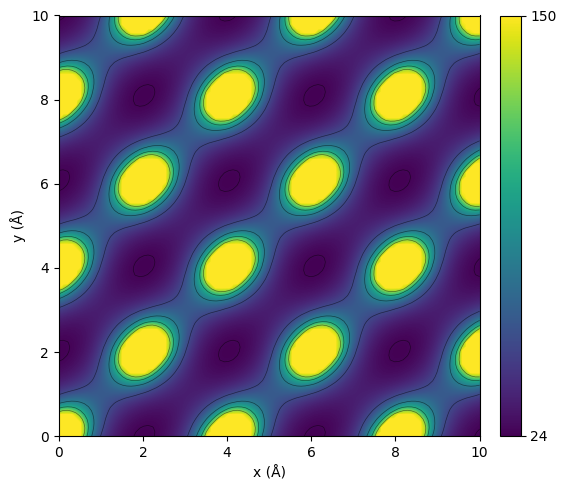
\includegraphics[width=0.9\linewidth]{fig/sine_matrix.png}
    \caption{อันตรกิริยาแบบ Periodic ที่คำนวณด้วย Sine Matrix}
    \label{fig:sine_matrix}
\end{figure}

%--------------------------
\subsection{Ewald Sum Matrix}
\label{ssec:ewald_sum_matrix}
\idxen{Representation!Ewald Sum Matrix}
%--------------------------

Ewald Sum Matrix เป็น Representation ที่พัฒนาต่อมาจาก Coulomb Matrix ซึ่งได้รวมผลของอันตรกิริยาระหว่างอะตอมแบบ Periodic 
โดยใช้อันตรกิริยาไฟฟ้าสถิตย์เข้าไปด้วย\autocite{faber2015}

\begin{equation}\label{eq:ewald_sum}
    \phi^{\text{self}}_{ij} + \phi^{\text{bg}}_{ij} = -\frac{\alpha}{\sqrt{\pi}}(Z_i^2 + Z_j^2) 
    -\frac{\pi}{2V\alpha^2}(Z_i + Z_j)^2~\forall~i \neq j
\end{equation}

\noindent โดยที่ $\phi^{\text{bg}}_{ij}$ คือ Background Charge

ตัวอย่างของโค้ดสำหรับการคำนวณ Ewald Sum Matrix

\begin{lstlisting}[style=MyPython]
from dscribe.descriptors import EwaldSumMatrix

atomic_numbers = [1, 8]
rcut = 6.0
nmax = 8
lmax = 6

# Setting up the Ewald sum matrix descriptor
esm = EwaldSumMatrix(
    n_atoms_max=6,
)
\end{lstlisting}

%--------------------------
\subsection{Bag of Bonds}
\label{ssec:bob}
\idxen{Representation!Bag of Bonds}
%--------------------------

นอกจากนี้ยังมี Bag of Bonds (BoB)\autocite{hansen2015} ซึ่งเป็น Representation ที่พัฒนาต่อจาก Coulomb Matrix 
โดยจะมีการจัดกลุ่มประเภทของพันธะเข้าด้วยกัน ซึ่งได้แรงบันดาลใจในการพัฒนามาจาก Bag of Words ที่ใช้ใน Natural Language Processing
(NLP) โดยคำว่า \textit{Bag} ในที่นี้คือประเภทของพันธะเคมีที่แตกต่างกันในโมเลกุลนั้น ๆ เช่น \ce{C-C}, \ce{C-O}, และ \ce{C-H} 
ส่วน \textit{Bond} นั้นจะแยกตามชนิดของพันธะ คือพันธะเดี่ยว พันธะคู่ และพันธะสาม

ตัวอย่างโค้ดของการคำนวณ Bag of Bonds ของโมเลกุล Methane\footnote{พิกัดคาร์ทีเซียนดูได้ที่ 
\url{https://en.wikipedia.org/wiki/Z-matrix_(chemistry)}} โดยใช้ไลบรารี่ qml\autocite{zotero-1799} 
โดยสามารถดูรายละเอียดเพิ่มเติมได้ที่\footnote{https://www.qmlcode.org}

\begin{lstlisting}[style=MyPython]
>>> import qml
>>> CH4 = qml.Compound(xyz="methane.xyz")
>>> CH4.generate_bob(asize={"C":4, "H":8})
>>> print(CH4.representation)
[36.8581052   0.          0.          0.          0.          0.          0.          0.
  0.          0.          5.50964209  5.50964187  5.50963981  5.50963981  0.          0.
  0.          0.          0.          0.          0.          0.          0.          0.
  0.          0.          0.          0.          0.          0.          0.          0.
  0.          0.          0.          0.          0.          0.          0.          0.
  0.          0.          0.5         0.5         0.5         0.5         0.          0.
  0.          0.          0.56232548  0.56232539  0.56232539  0.56232533  0.56232532  0.56232532
  0.          0.          0.          0.          0.          0.          0.          0.
  0.          0.          0.          0.          0.          0.          0.          0.
  0.          0.          0.          0.          0.          0.        ]
\end{lstlisting}

%--------------------------
\section{ลักษณะเฉพาะเชิงอิเล็กทรอนิกส์สำหรับอะตอม}
\label{sec:elec_feat}
\idxth{ลักษณะเฉพาะ!เชิงอิเล็กทรอนิกส์สำหรับอะตอม}
\idxen{Representation!Electronic Descriptor}
%--------------------------

นอกเหนือจาก Representation ที่เรานำมาอธิบายโมเลกุลแบบทั้งโมเลกุล ยังมี Representation แบบอื่นซึ่งมีความซับซ้อนมากกว่าที่ถูกพัฒนา%
ขึ้นมาเพื่ออธิบาย Environment ของโมเลกุลในระดับอะตอมแบบเฉพาะเจาะจง ซึ่ง Representation แบบนี้จะเป็นการรวมความสำคัญของกฎทาง%
ฟิสิกส์และเคมีแบบต่าง ๆ เข้ามาไว้ด้วยกัน จึงทำให้ Representation ประเภทนี้มีความสามารถในการที่จะอธิบายโครงสร้างเชิงอิเล็กทรอนิกส์ของ%
โมเลกุลได้ดีมาก ๆ โดยเฉพาะการทำนายคุณสมบัติในระดับอะตอม โดยในปัจจุบันก็ได้มีการพัฒนา Representation ที่สามารถอธิบายอะตอมแบบ%
ทีละอะตอม ซึ่งเราเรียก Representation ประเภทนี้ว่า Atom-wise ดังนั้นผู้เขียนจะขออธิบายเฉพาะ Representation ที่มีความโดดเด่นน่าสนใจ%
และเป็นที่นิยมในการนำมาใช้ในงานวิจัยเท่านั้น

การพัฒนา Representation สำหรับอธิบายโครงสร้างเชิงอิเล็กทรอนิกส์ของโมเลกุลนั้นสามารถใช้องค์ความรู้ที่เกี่ยวข้องกับความหนาแน่น (Density)
ของโมเลกุล\autocite{yang1991}, เทคนิค Linear Scaling ในเชิงคำนวณ\autocite{galli1992,goedecker1999}, หลักการมองเห็น%
ระยะสั้น (Nearsightedness Principle)\autocite{prodan2005} รวมไปถึงการพิจารณาสมมาตร (Symmetry) ของโมเลกุล เพื่อมาใช้ใน%
การออกแบบและปรับปรุงประสิทธิภาพของ Representation เพื่อให้ครอบคลุมและอธิบายปรากฏการณ์ทางควอนตัมให้ได้มากที่สุด%
\autocite{ceriotti2018}

%--------------------------
\subsection{Smooth Overlap of Atomic Positions}
\label{ssec:soap}
\idxen{Representation!Smooth Overlap of Atomic Positions}
%--------------------------

Representation ที่เป็นประเภทเชิงอิเล็กทรอนิกส์สำหรับอะตอมอันแรกที่จะพูดถึงก็คือ Smooth Overlap of Atomic Positions (SOAP) 
ซึ่งเป็นตัวที่โด่งดังมากแล้วก็มีการนำมาใช้อย่างแพ่หลาย เรียกได้ว่านักวิจัยเคมีควอนตัมและปัญญาประดิษฐ์ต่างก็รู้จัก SOAP กันเป็นอย่างดี
โดยบทความงานวิจัยของ SOAP ได้ถูกตีพิมพ์ครั้งแรกในปี ค.ศ. 2013 ซึ่งไอเดียของ SOAP ก็คือจะเป็นการนำข้อมูลโครงสร้างของอะตอมมาเข้ารหัส 
(Encoding) ไว้ได้โดยได้รวมสภาพแวดล้อมทางเคมีโดยการใช้ความหนาแน่นเชิงอะตอมแบบเกาส์เซียน (Gaussian Smeared Atomic Density) 
ซึ่ง Atomic Density ที่ว่านี้ก็ถูกคำนวณมาจากฟังก์ชันพื้นฐานเชิงรัศมี (Radial Basis Function, $g_{n}(r)$) และฟังก์ชันฮาร์โมนิคเชิงทรงกลม 
(Real Spherical Harmonic Functions, $Y_{lm}(\theta, \phi)$)\autocite{bartok2013,de2016}
โดย SOAP นั้นเหมาะสำหรับนำมาใช้ทำนายคุณสมบัติของโมเลกุลแบบเฉพาะที่ (Local Properties) อย่างเช่นแรงเชิงอะตอม (Atomic Force) 
หรือ Chemical Shift

การคำนวณ SOAP นั้นจริง ๆ แล้วสามารถทำได้ผ่านการคำนวณ Kernel ของ Atomic Environment 2 อันเข้าด้วยกัน ($\mathcal{X}$ และ 
$\mathcal{X}'$) ซึ่งเขียนออกมาได้ในรูปของ Polynomial Kernel ($K^\mathrm{SOAP}$ ของพารามิเตอร์ที่ชื่อว่า Partial Power 
Spectra ($\mathbf{p}$ และ $\mathbf{p}'$)\footnote{ผู้เขียนไม่แน่ใจว่าจะแปลเป็นภาษาไทยอย่างไรดี ต้องขออภัยผู้อ่านด้วยครับ} 

โดยสมการที่เรานำมาใช้ในการคำนวณ SOAP นั้นคือ

\begin{equation}\label{eq:soap}
    K^\mathrm{SOAP}(\mathbf{p}, \mathbf{p'}) = \left( \frac{\mathbf{p} \cdot \mathbf{p'}}{\sqrt{\mathbf{p} 
    \cdot \mathbf{p}~\mathbf{p'} \cdot \mathbf{p'}}}\right)^{\xi}
\end{equation}

\noindent โดยที่กำหนดให้ $\xi$ เป็นจำนวนเต็มบวกและสมาชิกของเวกเตอร์ $\mathbf{p}$ มีนิยามคือ 

\begin{equation}\label{eq:soap_power_spec}
    p^{Z_1 Z_2}_{n n' l} = \pi \sqrt{\frac{8}{2l+1}}\sum_m {c^{Z_1}_{n l m}}^{\dagger} c^{Z_2}_{n' l m}
\end{equation}

\noindent โดยที่ $n$ และ $n'$ เป็นดัชนีสำหรับ Radial Basis Function ซึ่งมีค่าได้สูงสุดถึง $n_{max}$, $l$ เป็นดีกรีเชิงมุม 
(Angular Degree) ของ Spherical Harmonics ซึ่งมีค่าได้สูงสุดถึง $l_{max}$, $m$ เป็นจำนวนเต็มที่สอดคล้องกับเงื่อนไขคือ $\abs{m} 
\leq l$, และ $Z_{1}$ และ $Z_{2}$ เป็นสปีชีส์เชิงอะตอม (Atomic Species) นอกจากนี้ค่าสัมประสิทธิ์ $c^{Z}_{n'lm}$ และ 
${c^{Z}_{nlm}}^{\dagger}$ ถูกนิยามให้เป็นผลคูณภายในของ Spherical Harmonic Functions กับความหนาแน่นเชิงอะตอมแบบเกาส์เซียน 
($\rho^Z$) และคอนจูเกตเชิงซ้อน (Complex Conjugate) ตามลำดับ\autocite{de2016} ดังนี้

\begin{equation}
    c^{Z}_{nlm}(\mathbf{r}) = \iiint_{\mathcal{R}^{3}} \mathrm{d}V g_{n}(r) Y_{lm}(\theta, \phi) 
    \rho^{Z}(\mathbf{r})
\end{equation}

\noindent โดยที่ $\mathbf{r}$ คือตำแหน่งในปริภูมิและ $\rho^Z(\mathbf{r})$ คือความหนาแน่นเชิงอะตอมแบบเกาส์เซียน (Gaussian 
Smoothed Atomic Density) สำหรับอะตอม $Z$ 

ในการคำนวณ $c^{Z}_{nlm}(\mathbf{r})$ นั้นเราจะต้องนั้นเราจะต้องมีการกำหนด Radial Basis Function (RBF) ที่เราต้องการใช้ด้วย 
โดยเราสามารถใช้ฟังก์ชัน Spherical Gaussian-type Orbitals (สมการที่ \ref{eq:rbf_gto}) หรือฟังก์ชัน Polynomial Basis 
(ตามสมการที่ \ref{eq:rbf_poly}) ก็ได้

\begin{equation}\label{eq:rbf_gto}
    g_{nl}(r) = \sum_{n'=1}^{n_\mathrm{max}}\,\beta_{nn'l} r^l e^{-\alpha_{n'l}r^2}
\end{equation}

\begin{equation}\label{eq:rbf_poly}
    g_{n}(r) = \sum_{n'=1}^{n_\mathrm{max}}\,\beta_{nn'} (r-r_\mathrm{cut})^{n'+2}
\end{equation}

\noindent และในส่วนของ Spherical Harmonics นั้นเราสามารถใช้เฉพาะส่วนจริง (Real Part) ได้ (เพราะว่าง่ายต่อการ Implement) 
โดยรูปแบบหรือสมการของ Spherical Harmonics มีดังนี้

\begin{align}\label{eq:spher_harmo}
    Y_{\ell m} &= \begin{cases}
    \dfrac{i}{\sqrt{2}} \left(Y_\ell^{m} - (-1)^m\, Y_\ell^{-m}\right) & \text{if}\ m < 0 \\
    Y_\ell^0 & \text{if}\ m=0 \\
    \dfrac{1}{\sqrt{2}} \left(Y_\ell^{-m} + (-1)^m\, Y_\ell^{m}\right) & \text{if}\ m > 0
    \end{cases} \\
    &= \begin{cases}
    \dfrac{i}{\sqrt{2}} \left(Y_\ell^{-|m|} - (-1)^{m}\, Y_\ell^{|m|}\right) & \text{if}\ m < 0 \\
    Y_\ell^0 & \text{if}\ m=0 \\
    \dfrac{1}{\sqrt{2}} \left(Y_\ell^{-|m|} + (-1)^{m}\, Y_\ell^{|m|}\right) & \text{if}\ m>0
    \end{cases} \\
    &= \begin{cases}
    \sqrt{2} \, (-1)^m \, \Im [{Y_\ell^{|m|}}] & \text{if}\ m<0 \\
    Y_\ell^0 & \text{if}\ m=0 \\
    \sqrt{2} \, (-1)^m \, \Re [{Y_\ell^m}] & \text{if}\ m>0
    \end{cases}
\end{align}

เนื่องจากว่ารายละเอียดในการพิสูจน์สมการ Kernel ของ SOAP นั้นมีความซับซ้อนพอสมควร ผู้เขียนจึงขอแนะนำให้ผู้อ่านที่สนใจศึกษาเพิ่มเติมทฤษฎีของ 
SOAP ได้ที่บทความต้นฉบับ\autocite{bartok2013}

ตัวอย่างโค้ดสำหรับการตั้งค่า SOAP Representation และคำนวณ SOAP ของโมเลกุลน้ำโดยใช้ไลบรารี่ DScribe และ ASE

\begin{lstlisting}[style=MyPython]
from dscribe.descriptors import SOAP
from ase.build import molecule

species = ["H", "C", "O", "N"]
r_cut = 6.0
n_max = 8
l_max = 6

# Setting up the SOAP descriptor
soap = SOAP(
    species=species,
    periodic=False,
    r_cut=r_cut,
    n_max=n_max,
    l_max=l_max,
)

# Molecule created as an ASE.Atoms
water = molecule("H2O")

# Create SOAP output for the system
soap_water = soap.create(water, positions=[0])

print(soap_water)
print(soap_water.shape)
\end{lstlisting}

\begin{figure}[htbp]
    \centering
    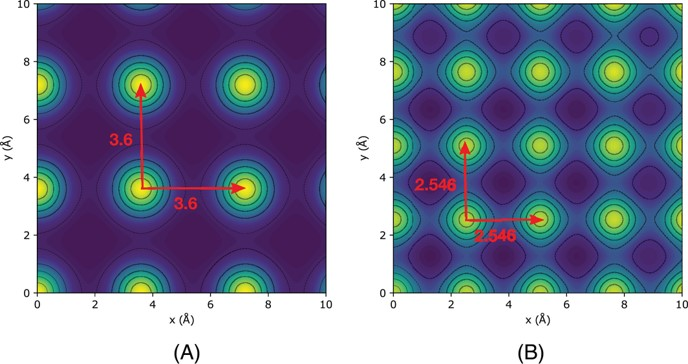
\includegraphics[width=\linewidth]{fig/soap_matrix.jpg}
    \caption{ตัวอย่างของ SOAP Matrix ของระบบ Cu/fcc Lattices สำหรับ (A) Cubic และ (B) Orthorhombic}
    \label{fig:soap_matrix}
\end{figure}

รายละเอียดเพิ่มเติมสำหรับการคำนวณและการเขียนโปรแกรมสำหรับคำนวณ SOAP นั้นสามารถดูได้ที่
\url{https://singroup.github.io/dscribe/latest/tutorials/descriptors/soap.html}

%--------------------------
\subsection{Atom-centered Symmetry Functions}
\label{ssec:acsf}
\idxen{Representation!Atom-centered Symmetry Functions}
%--------------------------

Representation ลำดับถัดมาคือฟังก์ชันสมมาตรแบบมีศูนย์กลางบนอะตอม (Atom-centered Symmetry Functions หรือ ACSF) เป็นวิธีที่ทำ%
การสร้างผลลัพธ์หรือคำตอบจากฟังก์ชันหลายวัตถุ (Many-body Functions) อีกทีหนึ่งเพื่อทำการประมาณค่า Electronic Environment รอบ ๆ 
อะตอมที่เราสนใจในโมเลกุล ซึ่ง ACSF นี้ได้ถูกพัฒนาโดยศาสตราจารย์ J\"{o}rg Behler ซึ่งตีพิมพ์ในปี ค.ศ. 2011 โดยถูกออกแบบเพื่อนำมา%
ใช้กับโมเดลประเภท Neuranl Network \autocite{behler2011a}

ไอเดียของ ACSF ก็คือจะเป็นการแปลง (Transformation) พิกัดคาร์ทีเซียนให้เป็น Symmetry Function โดยจะมีการกำหนดฟังก์ชันสำหรับ 
Cutoff ขึ้นมาก่อน ดังนี้

\begin{equation}\label{eq:acsf_cutoff}
    f_{c}(R_{ij}) = 
    \begin{cases}
        \frac{1}{2}[\cos(\frac{\pi R_{ij}}{R_{c}}) + 1], & R_{ij} \le R_{c} \\
        0,                                             & R_{ij} \ge R_{c}
    \end{cases}
\end{equation}

\noindent โดยที่ $R_{ij}$ คือระยะห่างระหว่างอะตอม $i$ กับ $j$ และ $R_{c}$ คือค่า Cutoff

สำหรับ Symmetry Function ทั้งหมดที่เราสามารถนำมาคำนวณออกมาเป็น Descriptor ได้นั้นจะมีประเภทนั่นคือฟังก์ชันแบบสองวัตถุ
(Two-body Function) และฟังก์ชันแบบสามวัตถุ (Three-body Function) นั่นก็คือฟังก์ชันเชิงรัศมี (Radial Function) และฟังก์ชันเชิงมุม 
(Angular Function) ตามลำดับ โดยเรามาดูกันที่ Radial Function ก่อนซึ่งจะมีด้วยกัน 3 แบบย่อย ดังนี้

\begin{equation}\label{eq:rf_g1}
    G^{1}_{i} = \sum_{j} f_{c}(R_{ij})
\end{equation}

\begin{equation}\label{eq:rf_g2}
    G^{2}_{i} = \sum_{j} e^{-\eta(R_{ij} - R_{s})^{2}} f_{c}(R_{ij})
\end{equation}

\begin{equation}\label{eq:rf_g3}
    G^{3}_{i} = \sum_{j} \cos(\kappa R_{ij}) f_{c}(R_{ij})
\end{equation}

\noindent ซึ่ง $G^{1}_{i}$ ก็คือฟังก์ชันผลรวมของ Cutoff Function (\ref{eq:acsf_cutoff}), $G^{2}_{i}$ คือผลรวม Gaussian 
Function คูณด้วย Cutoff Function และ $G^{3}_{i}$ คือฟังก์ชัน Cosine ที่ถูกปรับการหน่วงโดยค่าพารามิเตอร์ $\kappa$ 

นอกจากนี้ยังมี Angular Function อีกสองอันย่อยด้วยกัน ดังนี้

\begin{align}\label{eq:rf_g4}
    G^{4}_{i} =~&2^{1 - \xi}\sum^{\text{all}}_{j,k \neq i} (1+\lambda \cos \theta_{ijk})^{\xi}
    \cdot e^{-\eta(R^{2}_{ij} + R^{2}_{ik} + R^{2}_{jk})} \nonumber \\
    & \cdot f_{c}(R_{ij}) \cdot f_{c}(R_{ik}) \cdot f_{c}(R_{jk})
\end{align}

\noindent และ

\begin{align}\label{eq:rf_g5}
    G^{5}_{i} =~&2^{1 - \xi}\sum^{\text{all}}_{j,k \neq i} (1+\lambda \cos \theta_{ijk})^{\xi}
    \cdot e^{-\eta(R^{2}_{ij} + R^{2}_{ik})} \nonumber \\
    & \cdot f_{c}(R_{ij}) \cdot f_{c}(R_{ik}))
\end{align}

สำหรับการคำนวณหาแรง (Force) และเทนเซอร์แรงผลัก (Stress Tensor) สำหรับกรณีของ ACSF นั้นสามารถทำได้โดยใช้กฎลูกโซ่ (Chain 
Rule) ซึ่งต้องการทำพิสูจน์จากสมการของพลังงานที่เกิดขึ้นจากการคำนวณใน Neural Network โดยสำหรับค่าพลังงานย่อยต่อหนึ่งหน่วย Neuron 
นั้นมีนิยามตามนี้

\begin{equation}
    \label{eq:acsf_sub_ener}
    E_{\text{Neuron}} = f(w G + b) 
\end{equation}

\noindent โดยที่ $f$ คือฟังก์ชันกระตุ้น, $w$ คือค่าน้ำหนัก (Weight Parameter), $b$ คือค่าความอคติ (Bias Parameter) และ $G$ 
คืออินพุตของ Neuron นั้น ๆ ซึ่งก็คือ Symmetry Function ตามด้านบนที่ได้อธิบายไป โดยที่พลังงานรวมทั้งหมดของโมเลกุล (Total Energy, 
$E$) สามารถคำนวณได้จากผลรวมของพลังงานย่อย ๆ ที่เกิดขึ้นจากแต่ละอะตอม (สมการที่ \ref{eq:acsf_sub_ener}) ซึ่งมีสมการง่าย ๆ ดังนี้

\begin{equation}
    E = \sum_{i} E_{i}
\end{equation}

นอกจากนี้ยังมี Representation อื่น ๆ ที่คล้ายกับ ACSF นั่นคือถูกพัฒนาขึ้นมาด้วยไอเดีย Symmetry Function เหมือนกัน เช่น 
Spectrum of London and Axilrod-Teller-Muto (SLATM) ซึ่งถูกใช้อย่างแพร่หลายเหมือนกันแต่จะนิยมใช้กับ KRR มากกว่า%
\autocite{faber2018,huang2020} แล้วก็ยังมีการใช้ฟังก์ชันพหุนาม (Polynomial functions) ของส่วนกลับของระยะห่างระหว่างอะตอม
(Inverse Bond Distance) ด้วย\autocite{kwac2019,musil2021}

ตัวอย่างโค้ดสำหรับการตั้งค่า ACSF Representation และคำนวณ ACSF ของโมเลกุลน้ำโดยใช้ไลบรารี่ DScribe และ ASE

\begin{lstlisting}[style=MyPython]
from dscribe.descriptors import SOAP
from ase.build import molecule

# Setting up the ACSF descriptor
acsf = ACSF(
    species=["H", "O"],
    rcut=6.0,
    g2_params=[[1, 1], [1, 2], [1, 3]],
    g4_params=[[1, 1, 1], [1, 2, 1], [1, 1, -1], [1, 2, -1]],
)

# Molecule created as an ASE.Atoms
water = molecule("H2O")

# Create ACSF output for the hydrogen atom at index 1
acsf_water = acsf.create(water, positions=[1])

print(acsf_water)
print(acsf_water.shape)
\end{lstlisting}

%--------------------------
\subsection{Gaussian-type Orbital-based Density Vectors}
\label{ssec:gauss_orb_den}
\idxen{Representation!Gaussian-type Orbital-based Density Vectors}
%--------------------------

เวกเตอร์ของความหนาแน่นเชิงออร์บิทัลประเภทเกาส์เซียน (Gaussian-type Orbital-based Density Vector หรือเรียกสั้น ๆ ว่า GTB-based 
Density Vector) เป็น Representation อีกอันหนึ่งที่ใช้หลักการของ Molecular/Atomic Orbitals ซึ่งถูกพัฒนาขึ้นมาเพื่อให้เป็นอีกทาง%
เลือกหนึ่งนอกเหนือจาก ACSF และ Symmstric Polynomial Function\autocite{kwac2021} โดยสมการที่ใช้คำนวณ GTO-based Density 
Vector คือ

\begin{equation}
    \rho^{i}_{L,\alpha,r_{s}} = \sum^{l_{x}+l_{y}+l_{z} = L}_{l_{x},l_{y},l_{z}} 
    \frac{L!}{l_{x}!l_{y}!l_{z}!} \left ( \sum^{n_{type}}_{t=1} c_{t} \sum^{N^{t}_{atom}}_{j=1} 
    \phi^{\alpha,r_{s}}_{l_{x}l_{y}l_{z}} (\bm{r}_{ij}) \right )
\end{equation}

\noindent โดยกำหนดให้ $l_{x}+l_{y}+l_{z} = L$ เป็นเลข Angular Momentum ของออร์บิทัล, $n_{type}$ เป็นชนิดของอะตอมใน%
โมเลกุล, $c_{t}$ เป็นค่าถ่วงน้ำหนักที่ขึ้นกับชนิดของอะตอม (Type-dependent Weight), $N^{t}_{atom}$ คือจำนวนของอะตอมชนิด%
นั้น ๆ และ $\phi^{\alpha,r_{s}}_{l_{x}l_{y}l_{z}} (r_{ij})$ เป็นออร์บิทัลแบบเกาส์เซียนของแต่ละอะตอม นอกจากนี้ยังมีการกำหนด%
พารามิเตอร์เพิ่มเติมคือ $\alpha$ และ $r_{s}$ ซึ่งเป็นตัวกำหนดฟังก์ชันออร์บิทัลของ Radial Distribution

\begin{equation}
    \phi^{\alpha,r_{s}}_{l_{x}l_{y}l_{z}} (\bm{r}_{ij}) = x^{l_{x}}y^{l_{y}}z^{l_{z}} e^{-\alpha 
    |r-r_{s}|^{2}}
\end{equation}

\noindent โดยกำหนดให้ $\bm{r}_{ij} = (x,y,z)$ แสดงถึงเวกเตอร์จากอะตอม $i$ ไปยังอะตอม $j$ และ $r$ 
เป็นขนาด (Magnitude) ของ $\bm{r}_{ij}$ โดยทั่วไปแล้วเรามักจะกำหนดให้ค่า $L=0,1$ สำหรับการสร้าง Density Vector 
ด้วย GTO สำหรับโมเลกุลขนาดเล็ก เช่น โมเลกุลเคมีอินทรีย์ที่ประกอบไปด้วยอะตอมขนาดเล็ก เช่น คาร์บอน (C), ไฮโดรเจน (H), ออกซิเจน 
(O), และไนโตรเจน (N)\autocite{kwac2021}

%--------------------------
\subsection{ลักษณะเฉพาะเชิงอิเล็กทรอนิกส์อื่น ๆ}
\label{ssec:other_feat_elec}
%--------------------------

นอกจากนี้ยังมีลักษณะเฉพาะเชิงอิเล็กทรอนิกส์อีกมากมายที่ถูกพัฒนาขึ้นมา\autocite{faber2018} ดังนี้ 

\begin{itemize}[topsep=0pt]
    \item Bonds and Angles based Machine Learning (BAML)\autocite{huang2016}

    \item Histogram of Distances, Angles, and Dihedrals (HDAD)\autocite{faber2017}

    \item Many-body Tensor Representation (MBTR)\autocite{huo2022,langer2022}
    
    \item Faber-Christensen-Huang-Lilienfeld (FCHL)\autocite{faber2018}
    
    \item Atomic Cluster Expansion (ACE)\autocite{drautz2019,kovacs2021}
    
    \item N-body iterative contraction of equivariants (NICE)\autocite{nigam2020}
\end{itemize}

เมื่ออ่านบทความวิจารณ์ (Review) ต่าง ๆ แล้วผู้อ่านจะพบว่าไม่มี Descriptor ไหนที่ให้ผลการทำนายคุณสมบัติเชิงโมเลกุลทุกคุณสมบัติได้แม่น%
ยำที่สุด กล่าวคือ Descriptor แต่ละอันนั้นมีความสามารถในการทำนายคุณสมบัติที่แตกต่างกันไป ถ้าเปรียบเทียบง่าย ๆ ก็เหมือนกับ Functional 
ของวิธี DFT ซึ่งแต่ละ Functional ก็มีข้อดีและข้อเสียแตกต่างกันไป ดังนั้นผู้เขียนควรศึกษาความแตกต่างของ Descriptor แต่ละอันว่ามีทฤษฎี%
ที่อยู่เบื้องหลังที่ใช้ในการพัฒนา Descriptor นั้น ๆ เป็นอย่างไร จะช่วยทำให้เราเข้าใจและสามารถเลือกใช้ Descriptor ที่เหมาะกับคุณสมบัติ%
เชิงโมเลกุลได้อย่างเหมาะสมและให้ผลการทำนายที่ถูกต้องและแม่นยำ ซึ่งจะช่วยประหยัดเวลาโดยไม่ต้องทำการสุ่มหรือทดลองเปลี่ยน Descriptor 
ไปเรื่อย ๆ นั่นเอง

นอกจากนี้ผู้เขียนขอแนะนำผู้อ่านที่สนใจการศึกษา Descriptor แบบเชิงลึกได้อ่านบทความงานวิจัย \enquote{Physics-Inspired Structural 
Representations for Molecules and Materials}\autocite{musil2021} ที่ได้สรุป Descriptor (ในบทความต้นฉบับผู้วิจัยใช้คำว่า 
Representation ซึ่งเป็นสิ่งเดียวกัน) ที่เกี่ยวข้องกับ Atomic Composition สำหรับศึกษาคุณสมบัติเชิงเคมีควอนตัมของโมเลกุลไว้อย่างครบถ้วน 
รวมไปถึงสรุปคุณสมบัติของ Descriptor ที่ดีไว้ด้วย
